%%
%% ****** ljmsamp.tex 13.06.2018 ******
%%
\documentclass[
11pt,%
tightenlines,%
twoside,%
onecolumn,%
nofloats,%
nobibnotes,%
nofootinbib,%
superscriptaddress,%
noshowpacs,%
centertags]%
{revtex4}
\usepackage{ljm}

\usepackage[utf8]{inputenc}
\usepackage[russian]{babel}

\begin{document}

\titlerunning{Surface remesh methods} % for running heads
\authorrunning{Rybakov} % for running heads
%\authorrunning{First-Author, Second-Author} % for running heads

\title{Оценки методов перестроения поверхности \\ в задаче ледообразования}
% Splitting into lines is performed by the command \\
% The title is written in accordance with the rules of capitalization.

\author{\firstname{А.~А.}~\surname{Рыбаков}}
\email[E-mail: ]{rybakov_aan@nrcki.ru,rybakov@jscc.ru,rybakov.aax@gmail.com}
\affiliation{Национальный исследовательский центр «Курчатовский институт», 123182, Москва, пл. Академика Курчатова, д. 1, Россия.}

%\author{\firstname{B.}~\surname{Second-Author}}
%\email[E-mail: ]{Second.Author@email.com}
%\affiliation{Place of work and/or the address of the first and second authors}
%\affiliation{Place of work and/or the address of second authors}
%\noaffiliation % If the author does not specify a place of work.

\firstcollaboration{(Submitted by TODO)} % Add if you know submitter.
%\lastcollaboration{ }

%\received{June 13, 2018} % The date of receipt to the editor, i.e. December 06, 2017

\begin{abstract} % You shouldn't use formulas and citations in the abstract.
В статье рассматривается проблема перестроения поверхностной расчетной сетки в задаче ледообразования.
В этой задаче поверхностная сетка должна быть перестроена в соответствии с объемом накопленного льда в каждой ячейке сетки.
Главным фактором при выборе метода перестроения сетки является точность метода, характеризующаяся величиной отклонения заметаемого ячейкой объема от целевого значения.
Другим определяющим фактором является способность метода перестроения сглаживать дефекты сетки -- острые пики и впадины.
Без этого расчетная сетка может накапливать дефекты, что рано или поздно приводит к невозможности продолжения расчетов.
В работе рассматриваются теоретические оценки трех методов перестроения поверхностной сетки -- метода прямоугольников, метода трапеций и метода окрестностей -- с точки зрения точности перестроения и способности сглаживания дефектов.
Результаты анализа показали, что методы прямоугольников и трапеций не могут сглаживать дефекты расчетной сетки при перестроении, а значит их использование в задаче ледообразования небезопасно.
Метод окрестностей обладает допустимой точностью перестроения и может сглаживать дефекты расчетной сетки.
Все результаты получены в двумерной постановке, однако выводы могут быть перенесены на аналогичные методы перестроения поверхностной сетки в трехмерном случае.
\end{abstract}

\subclass{68U05} % Enter 2010 Mathematics Subject Classification.

\keywords{перестроение поверхностной сетки, метод прямоугольников, метод трапеций, метод окрестностей, точность перестроения, сглаживание острых пиков и впадин} % Include keywords separeted by comma.

\maketitle

% Text of article starts here.

%--------------------------------------------------------------------------------------------------------------------------------

\section{Introduction}

Численное моделирование процесса обледенения поверхности тела является сложной мультифизической задачей, включающей в себя моделирование процессов газовой динамики, теплообмена, течения жидкости, динамики капель в воздушном потоке и других.
Исследование процессов ледообразования имеет важное практическое значение.
В частности характер и интенсивность образования льда на поверхности летательного аппарата критическим образом влияет на его летные характеристики, что напрямую связано с безопасностью полетов \cite{Raj}.

На сегодняшний день среди зарубежного программного обеспечения для моделирования процесса ледообразования лидером является программный комплекс ANSYS (включая модули FENSAP-ICE, DROP3D, ICE3D) \cite{Martini}.
В России также активно ведется разработка математических алгоритмов и программного обеспечения по этому направлению.
Можно отметить исследования по разработке модуля iceFoam в составе открытого пакета OpenFOAM \cite{Koshelev}.
Среди коммерческих продуктов в последние годы активно развивается пакет IceVision в составе программного комплекса FlowVision \cite{Sorokin}, а также решение в составе пакета инженерного анализа ЛОГОС \cite{Galanov}.

Моделирование процесса ледяного покрова осуществляется, как правило, на поверхностной расчетной сетке и состоит из двух основных частей.
Первой частью является вычисление интенсивности нарастания льда в отдельных элементах сетки (это может быть вычисление массы скопившегося льда в каждой ячейке расчетной сетки за единицу времени, либо скорость образования ледяного покрова в узлах сетки, либо другие аналогичные характеристики).
Для выполнения вычисления интенсивности нарастания льда в элементах расчетной сетки существует множество моделей ледообразования, учитывающих разные состояния льда, динамику водяной пленки, тепловые потоки и другие факторы \cite{Bartkus,Zhang,Pena}.
Модели ледообразования не рассматриваются в рамках данной работы.
Второй важной составляющей моделирования ледяного нароста является определение изменения поверхности тела после нарастания на ней слоя льда.
В данной статье проводится анализ методов перестроения поверхностной сетки в двумерной постановке, для которых существуют трехмерные аналоги.

Рассмотрим геометрическую задачу о перестроении поверхности в двумерном пространстве в общем виде.
Пусть дана поверхностная сетка в виде ломаной без самопересечений, каждая ячейка которой представлена отрезком длины $l_i$ ($0 \le i < n$).
У $i$-ой ячейки инцидентными узлами являются узлы с номерами $i$ и $i + 1$.
Если узлы с номерами $0$ и $n$ совпадают, то сетка является замкнутой.
Известно направление нормали каждой ячейки, а также направление движения каждого узла, совпадающее с направлением суммы единичных нормалей, проведенных к инцидентным ячейкам.
Для двумерного случая это направление лежит на биссектрисе угла, образованного двумя инцидентными ячейками.
Угол между двумя соседними ячейками с номерами $i - 1$ и $i$ будем обозначать через $2 \phi_i$.
Пусть известно, что за некий малый промежуток времени $i$-ая ячейка сдвигается в направлении своей нормали на некоторую величину $H_i$, заметая таким образом площадь $T_i = l_i H_i$, эту площадь будем называть целевой площадью.
Однако если просто сдвинуть каждую ячейку в направлении своей нормали, то сетка потеряет целостность, поэтому мы можем осуществлять движение только узлов.
Требуется найти такие значения локальных сдвигов узлов сетки $h_i$ ($0 \le i \le n$), чтобы заметаемая площадь $S_i$ между исходной поверхностью и новой поверхностью для каждой ячейки сетки как можно меньше отличалась от значения целевой площади $T_i$.
Для оценки отклонения фактической заметаемой площади от целевой будем использовать обозначения $\Delta_i = S_i - T_i$, $\delta_i = \frac{\Delta_i}{T_i}$.

В применении к задаче ледообразования величина $H_i$ соответствует толщине образозавшегося слоя льда в $i$-ой ячейке \cite{Beaugendre}.
Новая перестроенная поверхностная сетка соответствует поверхности ледяного покрова, а общая заметаемая площадь при движении поверхности соответствует объему накопленного на поверхности льда \cite{Tong}.
Задача нахождения величин сдвигов узлов сетки $h_i$ при фиксированных направлениях смещения может быть решена методом градиентного спуска \cite{Rybakov}.
Однако метод градиентного спуска оказывается слишком требовательным к вычислительным ресурсам при увеличении размера сетки.
К тому же, качество решения зачастую оказывается неудовлетворительным при попадании в локальные минимумы.
Поэтому для решения поставленной задачи могут быть использованы приближенные методы, основанные на представлении целевой площади в виде примитивных геометрических фигур.

%--------------------------------------------------------------------------------------------------------------------------------

\section{Приближенные методы перестроения поверхности}

Рассмотрим приближенные методы перестроения расчетной сетки, основанные на представлении целевой площади в виде примитивных геометрических фигур.

\begin{figure}[ht]
\setcaptionmargin{5mm}
%\onelinecaptionsfalse % if the caption is multiline
\onelinecaptionstrue  % if the caption is one-line
\begin{tabular}{ll}
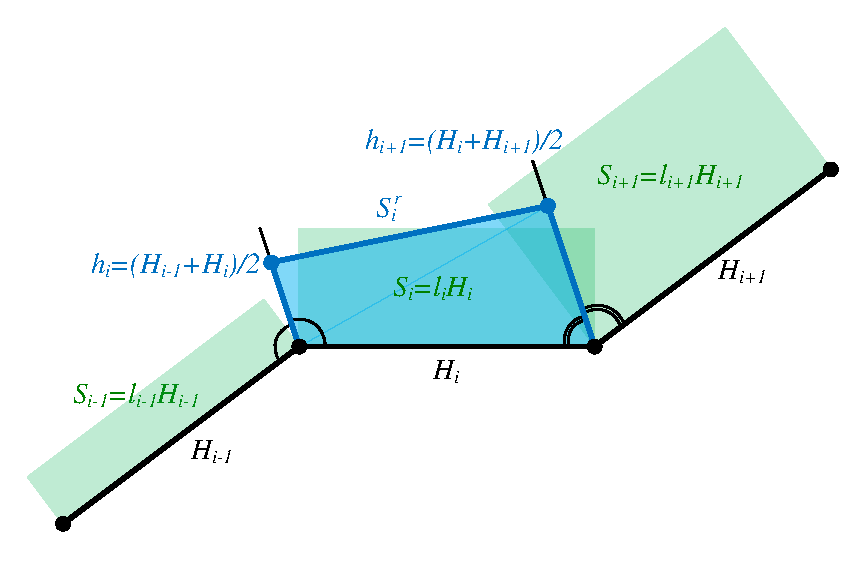
\includegraphics[width=0.45\textwidth]{pics/remesh_rectangles.pdf}
&
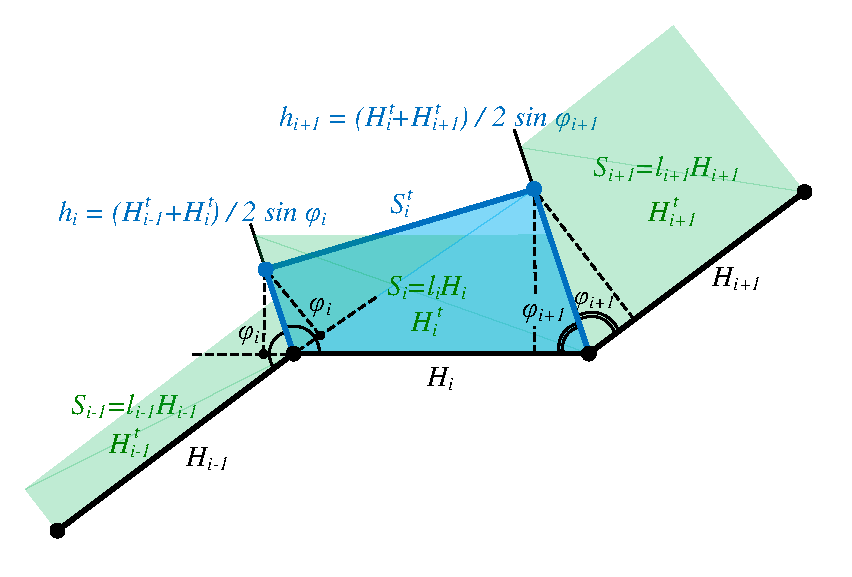
\includegraphics[width=0.45\textwidth]{pics/remesh_trapeziums.pdf}
\end{tabular}
\captionstyle{normal}\caption{Перестроение поверхности методом прямоугольников (слева) и трапеций (справа).}
\label{fig:text_1_remesh_2d_rectangles_and_trapeziums}
\end{figure}

В качестве первого метода перестроения поверхности рассмотрим приближение, при котором целевая площадь для $i$-ой ячейки представлена прямоугольником со сторонами $l_i$ и $H_i$.
В качестве величины смещения узла берется среднее арифметичское двух высот инцидентных ячеек $h_i = \frac{H_{i - 1} + H_i}{2}$ (см. рис.~\ref{fig:text_1_remesh_2d_rectangles_and_trapeziums} слева).
Этот метод перестроения поверхности будем называть методом прямогольников.
Заметаемую $i$-ой ячейкой площадь при использовании метода прямоугольников будем обозначать $S_i^r$, также обозначим $\Delta_i^r = S_i^r - T_i$, $\delta_i^r = \frac{\Delta_i^r}{T_i}$.

В качестве второго метода перестроения поверхности будем рассматривать метод трапеций.
В методе трапеций целевая площадь $i$-ой ячейки представляется трапецией с площадью $T_i = l_i H_i$.
Боковые стороны этой трапеции лежат на направлениях движения двух узлов, инцидентных рассматриваемой ячейке.
Высота трапеции $H_i^t$ находится с помощью решения квадратного уравнения.
После построения трапеций для всех ячеек сетки у каждого узла появляется две новые потенциальные позиции для сдвига (образованные ячейкой слева и ячейкой справа).
В качестве финальной новой позиции выбирается их среднее значение (рис.~\ref{fig:text_1_remesh_2d_rectangles_and_trapeziums} справа).
Таким образом, величина смещения узла определяется как $h_i = \frac{H_{i - 1}^t + H_i^t}{2 \sin \phi_i}$.
Заметаемую $i$-ой ячейкой площадь при использовании метода трапеций будем обозначать $S_i^t$, также обозначим $\Delta_i^t = S_i^t - T_i$, $\delta_i^t = \frac{\Delta_i^t}{T_i}$.

В качестве третьего метода перестроения сетки рассматривается метод окрестностей, описание которого в трехмерной постановке может быть найдено в \cite{Meshcheryakov}.
В этом методе для определения новых позиций узлов рассматривается фронт движения сетки (см. рис.~\ref{fig:text_1_remesh_2d_okrestnost}).

\begin{figure}[ht]
\setcaptionmargin{5mm}
%\onelinecaptionsfalse % if the caption is multiline
\onelinecaptionstrue  % if the caption is one-line
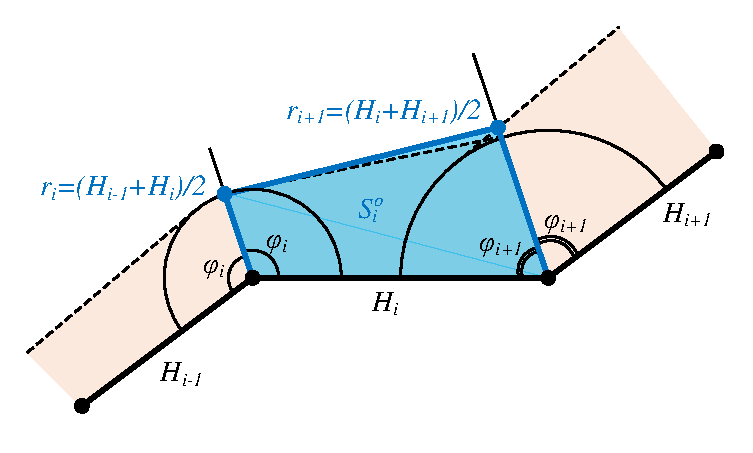
\includegraphics[width=0.6\textwidth]{pics/remesh_okrestnost.pdf}
\captionstyle{normal}\caption{Перестроение поверхности методом окрестностей.}
\label{fig:text_1_remesh_2d_okrestnost}
\end{figure}

При этом фронтом движения узла с номером $i$ является сфера с центром в этом узле и радиусом $r_i = \frac{H_{i - 1} + H_i}{2}$.
Фронтом движения ячейки сетки является выпуклая оболочка фронтов движения двух инцидентных ей узлов.
Тогда фронтом движения сетки является объединение фронтов движения всех ее ячеек.
В качестве нового положения узла будем брать пересечение направления смещения узла и границы фронта движения сетки.
Заметаемую $i$-ой ячейкой площадь при использовании метода окрестностей будем обозначать $S_i^o$, также обозначим $\Delta_i^o = S_i^o - T_i$, $\delta_i^o = \frac{\Delta_i^o}{T_i}$.

%--------------------------------------------------------------------------------------------------------------------------------

\section{Теоретические оценки точности методов перестроения сетки}

Приведем теоретическую оценку точности приближенных методов перестроения поверхности.
Оценку будем проводить для модельной расчетной сетки, которая удовлетворяет следующим требованиям.
Все ячейки сетки одинаковые и имеют длину $l$, поверхность является выпуклой.
Для любой ячейки $AB$ и ее соседей $A_2A$ и $BB_2$ углы $\angle (\overline{BA}, \overline{AA_2})$ и $\angle (\overline{AB}, \overline{BB_2})$ являются постоянной величиной и равны $\alpha$ (см. рис.~\ref{fig:text_1_remesh_2d_theoretical} слева).
Пусть величины смещений ячеек $A_2A$, $AB$ и $BB_2$ равны $H_{i - 1}$, $H_i$ и $H_{i + 1}$ соответственно.

\begin{figure}[ht]
\setcaptionmargin{5mm}
\onelinecaptionsfalse % if the caption is multiline
%\onelinecaptionstrue  % if the caption is one-line
\begin{tabular}{ll}
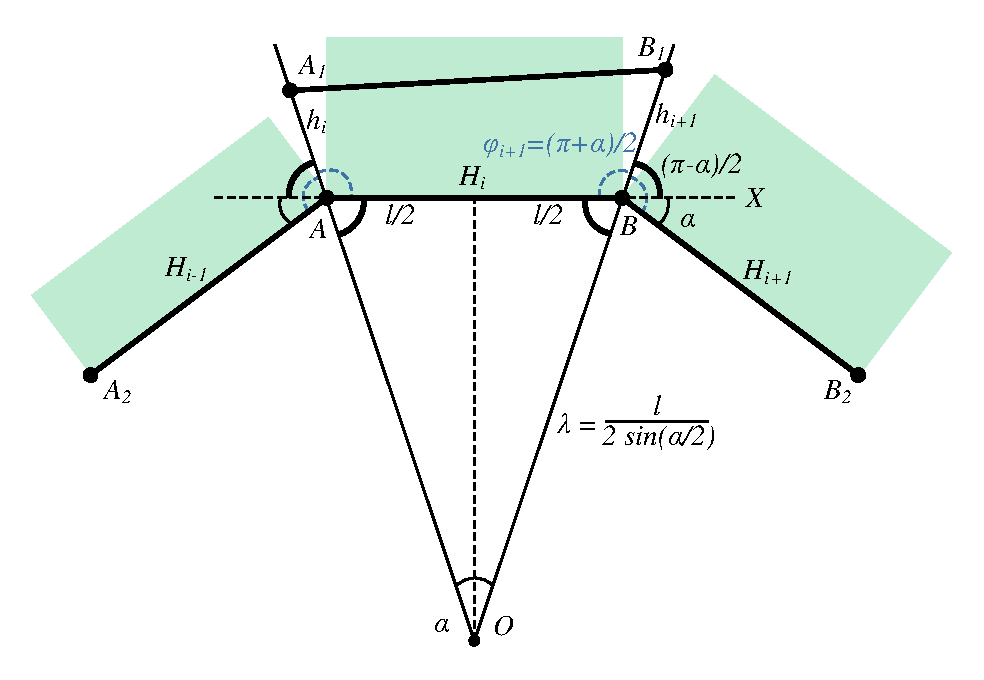
\includegraphics[width=0.45\textwidth]{pics/theoretical.pdf}
&
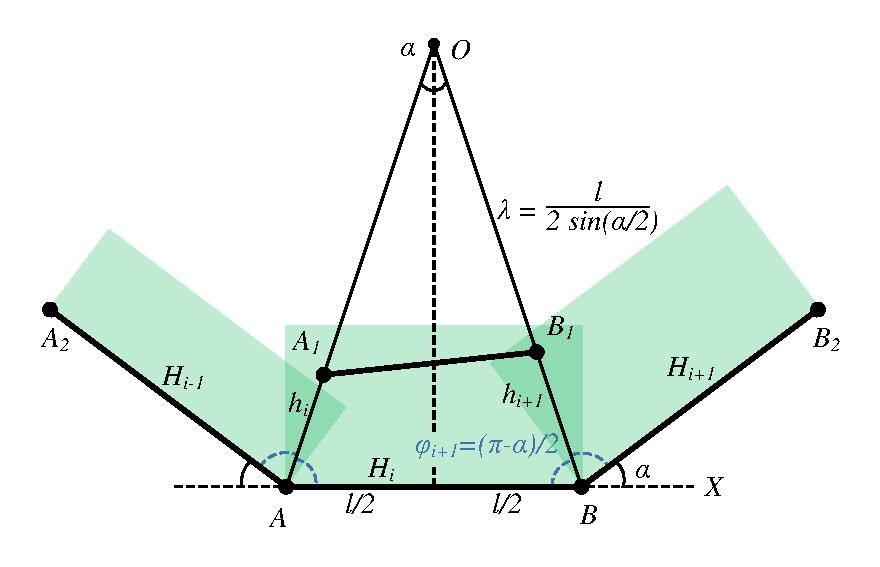
\includegraphics[width=0.45\textwidth]{pics/theoretical_concave.pdf}
\end{tabular}
\captionstyle{normal}\caption{Теоретическая оценка приближенных методов перестроения выпуклой (слева) и вогнутой (справа) сетки.}
\label{fig:text_1_remesh_2d_theoretical}
\end{figure}

Для вычисления величин $\Delta$, $\delta$ необходимо вычислить площадь $S_i = S_{AA_1B_1B}$.
При использовании разных методов перестроения эта площадь будет различаться.

\begin{lemma}\label{lem:text_1_remesh2_vypukl_lemma}
Для ячейки $AB$ выпуклой сетки с равными углами $\angle (\overline{BA}, \overline{AA_2}) = \angle (\overline{AB}, \overline{BB_2}) = \alpha$ (см. рис.~\ref{fig:text_1_remesh_2d_theoretical})
\begin{equation}\label{eqn:text_1_remesh2_saa2b2b_gen}
S_i(h_i, h_{i + 1}) = \frac{1}{2} \sin \alpha \left( \lambda(h_i + h_{i+1}) + h_ih_{i+1} \right)
\end{equation}
где $\lambda = \frac{l}{2 \sin \frac{\alpha}{2}}$, $l = AB$, $h_i = AA_1$, $h_{i + 1} = BB_1$.
\end{lemma}

Так как рассматриваемая сетка выпуклая, то лучи $A_1A$ и $B_1B$ пересекаются в некоторой точке $O$.
При этом треугольник $AOB$ равнобедренный, $\angle BAO = \angle ABO = \angle B_1BX = \angle B_1BB_2 - \alpha = \frac{\pi - \alpha}{2}$, $\phi_i = \phi_{i + 1} = \frac{\pi + \alpha}{2}$, $\angle AOB = \alpha$, откуда $OA = OB = \lambda = \frac{l}{2 \sin \frac{\alpha}{2}}$.
Далее выражаем площадь $S_i = S_{A_1OB_1} - S_{AOB}$, что после преобразования и дает требуемое соотношение \eqref{eqn:text_1_remesh2_saa2b2b_gen}.
$\blacksquare$\\

Далее будем рассматривать линейное изменение величины смещения ячеек сетки, то есть $H_i = H$, $H_{i - 1} = H - \Delta H$, $H_{i + 1} = H + \Delta H$.

Для перестроения методом прямоугольников имеем $h_i = H - \frac{1}{2} \Delta H$, $h_{i + 1} = H + \frac{1}{2} \Delta H$, откуда
\begin{equation}\label{eqn:text_1_remesh2_s_rect}
	S_i^r = \cos \frac{\alpha}{2} \left( lH + \left( H^2 - \frac{1}{4} \Delta H^2 \right) \sin \frac{\alpha}{2} \right)
\end{equation}

Теперь перейдем к вычислению $S_i^t$ для метода трапеций.
В методе трапеций мы должны представить целевые площади в ячейках $A_2A$, $AB$, $BB_2$ с помощью равнобоких трапеций, для которых известно одно из оснований (одинаково для всех ячеек и равно $l$), угол при этом основании (одинаковый для всех ячеек и равен $\phi = \frac{\pi + \alpha}{2}$, а также площади этих трапеций, равные $T_{i - 1} = l(H - \Delta H)$, $T_i = lH$ и $T_{i + 1} = l(H + \Delta H)$ соответственно.
На основании этих данных необходимо вычислить высоты трапеций, что можно сделать с помощью решения квадратного уравнения.
Обозначим высоты этих трапеций:
\begin{equation}
	\begin{aligned}\label{eqn:text_1_remesh_2_Ht_vypukl}
		& H_{i - 1}^t = H^t\left(l(H - \Delta H), l, \frac{\pi + \alpha}{2}\right) \\ 
		& H_i^t = H^t\left(lH, l, \frac{\pi + \alpha}{2}\right) \\
		& H_{i + 1}^t = H^t\left(l(H + \Delta H), l, \frac{\pi + \alpha}{2}\right)
	\end{aligned}
\end{equation}

Тогда $h_i = \frac{H_{i - 1}^t + H_i^t}{2 \sin \phi_i} = \frac{H_{i - 1}^t + H_i^t}{2 \cos \frac{\alpha}{2}}$, $h_{i+1} = \frac{H_i^t + H_{i+1}^t}{2 \sin \phi_{i + 1}} = \frac{H_i^t + H_{i+1}^t}{2 \cos \frac{\alpha}{2}}$ и выражение \eqref{eqn:text_1_remesh2_saa2b2b_gen} для $S_i^t$ принимает следующий вид:
\begin{equation}\label{eqn:text_1_remesh2_trap}
	S_i^t = \frac{1}{4} \left( (H_{i - 1}^t + 2 H_i^t + H_{i + 1}^t)l + (H_{i - 1}^t + H_i^t) (H_i^t + H_{i+1}^t) \tg \frac{\alpha}{2} \right)
\end{equation}

Для получения теоретической оценки точности для метода окрестностей в случае выпуклой сетки рассмотрим следующее вспомогательное утверждение (см. рис.~\ref{fig:text_1_remesh_2d_accuracy_okrestnost} слева).

\begin{figure}[ht]
\setcaptionmargin{5mm}
\onelinecaptionsfalse % if the caption is multiline
%\onelinecaptionstrue  % if the caption is one-line
\begin{tabular}{ll}
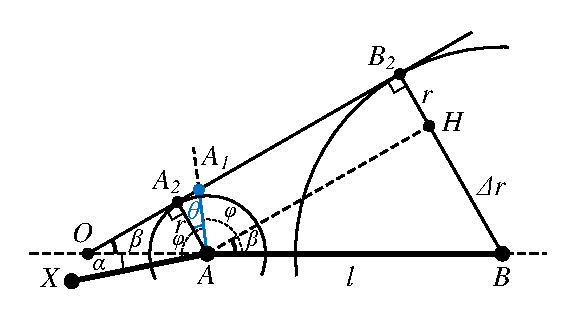
\includegraphics[width=0.45\textwidth]{pics/accuracy_okrestnost.pdf}
&
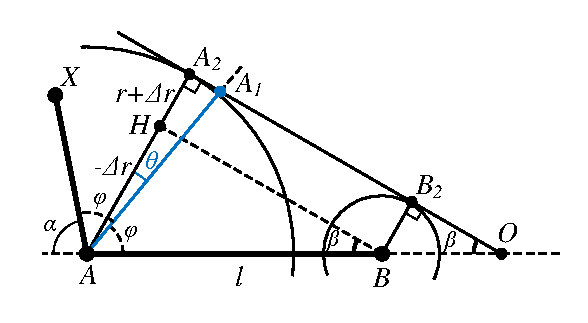
\includegraphics[width=0.45\textwidth]{pics/accuracy_okrestnost2.pdf}
\end{tabular}
\captionstyle{normal}\caption{Вычисление смещения узла в методе окрестностей для выпуклой (слева) и вогнутой (справа) сетки.}
\label{fig:text_1_remesh_2d_accuracy_okrestnost}
\end{figure}

\begin{lemma}\label{lem:text_1_remesh_2d_accuracy_okrestnost}
Пусть $AB = l$, ниже прямой $AB$ расположена точка $X$ такая, что $\angle (\overline{AX}, \overline{BA}) = \alpha$.
Пусть построены две окружности с центрами в точках $A$ и $B$ и с радиусами $r$ и $r + \Delta r$ соответственно.
Для построенных окружностей построена выпуклая оболочка, состоящая из дуг этих окружностей, а также отрезков общих касательных (точки касания общей касательной построенных окружностей, лежащие выше прямой $AB$, обозначим $A_2$ и $B_2$ соответственно).
Пусть на этой выпуклой оболочке -- на окружности с центром в точке $A$, либо на отрезке $A_2B_2$ -- лежит точка $A_1$ такая, что $\angle XAA_1 = \angle BAA_1 = \phi$, $AA_1 = h$, тогда 
\begin{equation}
	\begin{cases}\label{eqn:text_1_remesh_2d_okr_h}
		h = r, \  \sin \frac{\alpha}{2} > \frac{\Delta r}{l}, \\
		h(\alpha, l, r, \Delta r) = \frac{r}{\cos \left( \arcsin \frac{\Delta r}{l} - \frac{\alpha}{2} \right)}, \  \sin \frac{\alpha}{2} \le \frac{\Delta r}{l}
	\end{cases}
\end{equation}
\end{lemma}

Если точка $A_1$ не находится на отрезке $A_2B_2$, то $h = AA_1 = r$.

Рассмотрим случай, когда $A_1$ находится на отрезке $A_2B_2$, в этом случае $\Delta r > 0$.
Через точку $A$ проведем прямую, параллельную $A_2B_2$, до пересечения с $BB_2$ в точке $H$.
Тогда $\angle B_2OB = \angle HAB = \beta = \arcsin \frac{\Delta r}{l}$.
Так как $\angle A_1AB = \phi = \frac{\pi + \alpha}{2}$, то $\angle OAA_2 + \theta + \phi = \pi$, откуда получим $\theta = \beta - \frac{\alpha}{2}$.

Таким образом, условие нахождения точки $A_1$ на отрезке $A_2B_2$ равносильно $\theta \ge 0$.
То есть при $\theta < 0$, получаем $h = r$, а при $\theta \ge 0$ значение $h$ можно выразить из прямоугольного треугольника $AA_1A_2$.
$\blacksquare$\\

Используя лемму~\ref{lem:text_1_remesh_2d_accuracy_okrestnost}, для метода окрестностей можно выразить $S_i^o$ из \eqref{eqn:text_1_remesh2_saa2b2b_gen}, подставив туда выражения для $h_i$ и $h_{i + 1}$ из \eqref{eqn:text_1_remesh_2d_okr_h}:
\begin{equation}
	\begin{aligned}
	& h_i = h \left( \alpha, l, H - \frac{1}{2}\Delta H, \Delta H \right) \\
	& h_{i + 1} = h \left( \alpha, l, H + \frac{1}{2}\Delta H, \Delta H \right)
	\end{aligned}
\end{equation}

Теперь рассмотрим случай вогнутой сетки, представленный на рис.~\ref{fig:text_1_remesh_2d_theoretical} справа.

\begin{lemma}
Для ячейки $AB$ вогнутой сетки с равными углами $\angle (\overline{BA}, \overline{AA_2}) = \angle (\overline{AB}, \overline{BB_2}) = \alpha$ (см. рис.~\ref{fig:text_1_remesh_2d_theoretical} справа)
\begin{equation}\label{eqn:text_1_remesh2_saa2b2b_gen2}
S_i = \frac{1}{2} \sin \alpha \left( \lambda(h_i + h_{i+1}) - h_ih_{i+1} \right)
\end{equation}
где $\lambda = \frac{1}{2 \sin \frac{\alpha}{2}}$, $l = AB$, $h_i = AA_1$, $h_{i + 1} = BB_1$, при этом формула \eqref{eqn:text_1_remesh2_saa2b2b_gen2} применима при выполнении хотя бы одного из условий $h_i \le \lambda$, $h_{i+1} \le \lambda$.
\end{lemma}

Вычисления производятся аналогично лемме~\ref{lem:text_1_remesh2_vypukl_lemma}, с той лишь разницей, что $S_i = S_{AOB} - S_{A_1OB_1}$, откуда имеем выражение \eqref{eqn:text_1_remesh2_saa2b2b_gen2}.

Выполнение хотя бы одного из условий $h_i \le \lambda$, $h_{i+1} \le \lambda$ необходимо для предотвращения самопересечения сетки.
$\blacksquare$\\

Для перестроения методом прямоугольников и методом трапеций в случае вогнутой сетки получим формулы, аналогичные \eqref{eqn:text_1_remesh2_s_rect}, \eqref{eqn:text_1_remesh_2_Ht_vypukl} и \eqref{eqn:text_1_remesh2_trap}:
\begin{equation}\label{eqn:text_1_remesh2_s_rect_vogn}
	S_i^r = \cos \frac{\alpha}{2} \left( lH - \left( H^2 - \frac{1}{4} \Delta H^2 \right) \sin \frac{\alpha}{2} \right) \\
\end{equation}
\begin{equation}\label{eqn:text_1_remesh_2_Ht_vogn}
	\begin{aligned}
	& H_{i - 1}^t = H^t\left(l(H - \Delta H), l, \frac{\pi - \alpha}{2}\right) \\ 
	& H_i^t = H^t\left(lH, l, \frac{\pi - \alpha}{2}\right) \\
	& H_{i + 1}^t = H^t\left(l(H + \Delta H), l, \frac{\pi - \alpha}{2}\right)
	\end{aligned}
\end{equation}
\begin{equation}\label{eqn:text_1_remesh2_trap_vogn}
	S_i^t = \frac{1}{4} \left( (H_{i - 1}^t + 2 H_i^t + H_{i + 1}^t)l - (H_{i - 1}^t + H_i^t) (H_i^t + H_{i+1}^t) \tg \frac{\alpha}{2} \right)
\end{equation}

Заметим, что формулы \eqref{eqn:text_1_remesh2_s_rect_vogn} -- \eqref{eqn:text_1_remesh2_trap_vogn} идентичны формулам \eqref{eqn:text_1_remesh2_s_rect} -- \eqref{eqn:text_1_remesh2_trap} с учетом знака $\alpha$, поэтому формулы \eqref{eqn:text_1_remesh2_s_rect} -- \eqref{eqn:text_1_remesh2_trap} применимы как для положительных значений углов $\alpha$ (случай выпуклой сетки), так и для отрицательных значений $\alpha$ (случай вогнутой сетки).

Для получения теоретической оценки точности для метода окрестностей в случае вогнутой сетки рассмотрим следующее вспомогательное утверждение, аналогичное лемме~\ref{lem:text_1_remesh_2d_accuracy_okrestnost} (см. рис.~\ref{fig:text_1_remesh_2d_accuracy_okrestnost} справа).

\begin{lemma}\label{lem:text_1_remesh_2d_accuracy_okrestnost2}
Пусть $AB = l$, выше прямой $AB$ расположена точка $X$ такая, что $\angle (\overline{AX}, \overline{BA}) = \alpha$.
Пусть построены две окружности с центрами в точках $A$ и $B$ и с радиусами $r$ и $r + \Delta r$ соответственно.
Для построенных окружностей построена выпуклая оболочка, состоящая из дуг этих окружностей, а также отрезков общих касательных (точки касания общей касательной построенных окружностей, лежащие выше прямой $AB$, обозначим $A_2$ и $B_2$ соответственно).
Пусть на этой выпуклой оболочке -- на окружности с центром в точке $A$ либо на отрезке $A_2B_2$ -- лежит точка $A_1$ такая, что $\angle XAA_1 = \angle BAA_1 = \phi$, $AA_1 = h$, тогда 
\begin{equation}
	\begin{cases}\label{eqn:text_1_remesh_2d_okr_h2}
		h = r, \ \sin \frac{\alpha}{2} < \frac{-\Delta r}{l}, \\
		h(\alpha, l, r, \Delta r) = \frac{r}{\cos \left( \frac{\alpha}{2} - \arcsin \frac{-\Delta r}{l} \right)}, \ \sin \frac{\alpha}{2} \ge \frac{-\Delta r}{l}
	\end{cases}
\end{equation}
\end{lemma}

Если точка $A_1$ не находится на отрезке $A_2B_2$, то $h = AA_1 = r$.

Рассмотрим случай, когда $A_1$ находится на отрезке $A_2B_2$, в этом случае $\Delta r < 0$.
Через точку $B$ проведем прямую, параллельную $A_2B_2$, до пересечения с $AA_2$ в точке $H$.
Тогда $\angle A_2OA = \angle HBA = \beta = \arcsin \frac{-\Delta r}{l}$.
Так как $\angle A_1AB = \phi = \frac{\pi - \alpha}{2}$, то $\angle A_2AA_1 = \theta = \angle A_2AO - \phi = \frac{\alpha}{2} - \beta$.

Таким образом, условие нахождения точки $A_1$ на отрезке $A_2B_2$ равносильно $\theta \ge 0$.
То есть при $\theta < 0$, получаем $h = r$, а при $\theta \ge 0$ значение $h$ можно выразить из прямоугольного треугольника $AA_1A_2$.
$\blacksquare$\\

Используя лемму~\ref{lem:text_1_remesh_2d_accuracy_okrestnost2}, для метода окрестностей можно выразить $S_i^o$ из \eqref{eqn:text_1_remesh2_saa2b2b_gen2} подставив туда выражения для $h_i$ и $h_{i + 1}$ из \eqref{eqn:text_1_remesh_2d_okr_h2}:
\begin{equation}
	\begin{aligned}
	& h_i = \max \left( h \left( \alpha, l, H - \frac{3}{2}\Delta H, \Delta H \right), h \left( \alpha, l, H - \frac{1}{2}\Delta H, \Delta H \right) \right) \\
	& h_{i + 1} = \max \left( h \left( \alpha, l, H - \frac{1}{2}\Delta H, \Delta H \right), h \left( \alpha, l, H + \frac{1}{2}\Delta H, \Delta H \right) \right)
	\end{aligned}
\end{equation}

Используя полученные соотношения для $S_i^r$, $S_i^t$, $S_i^o$, можно проанализировать зависимости величин $\delta_i^r$, $\delta_i^t$, $\delta_i^o$ от $\alpha$ и $\frac{\Delta H}{l}$, при этом будем использовать фиксированную величину $H = \frac{l}{2}$ (см. рис.~\ref{fig:text_1_remesh_3d_main_chart}).

\begin{figure}[ht]
\setcaptionmargin{5mm}
%\onelinecaptionsfalse % if the caption is multiline
\onelinecaptionstrue  % if the caption is one-line
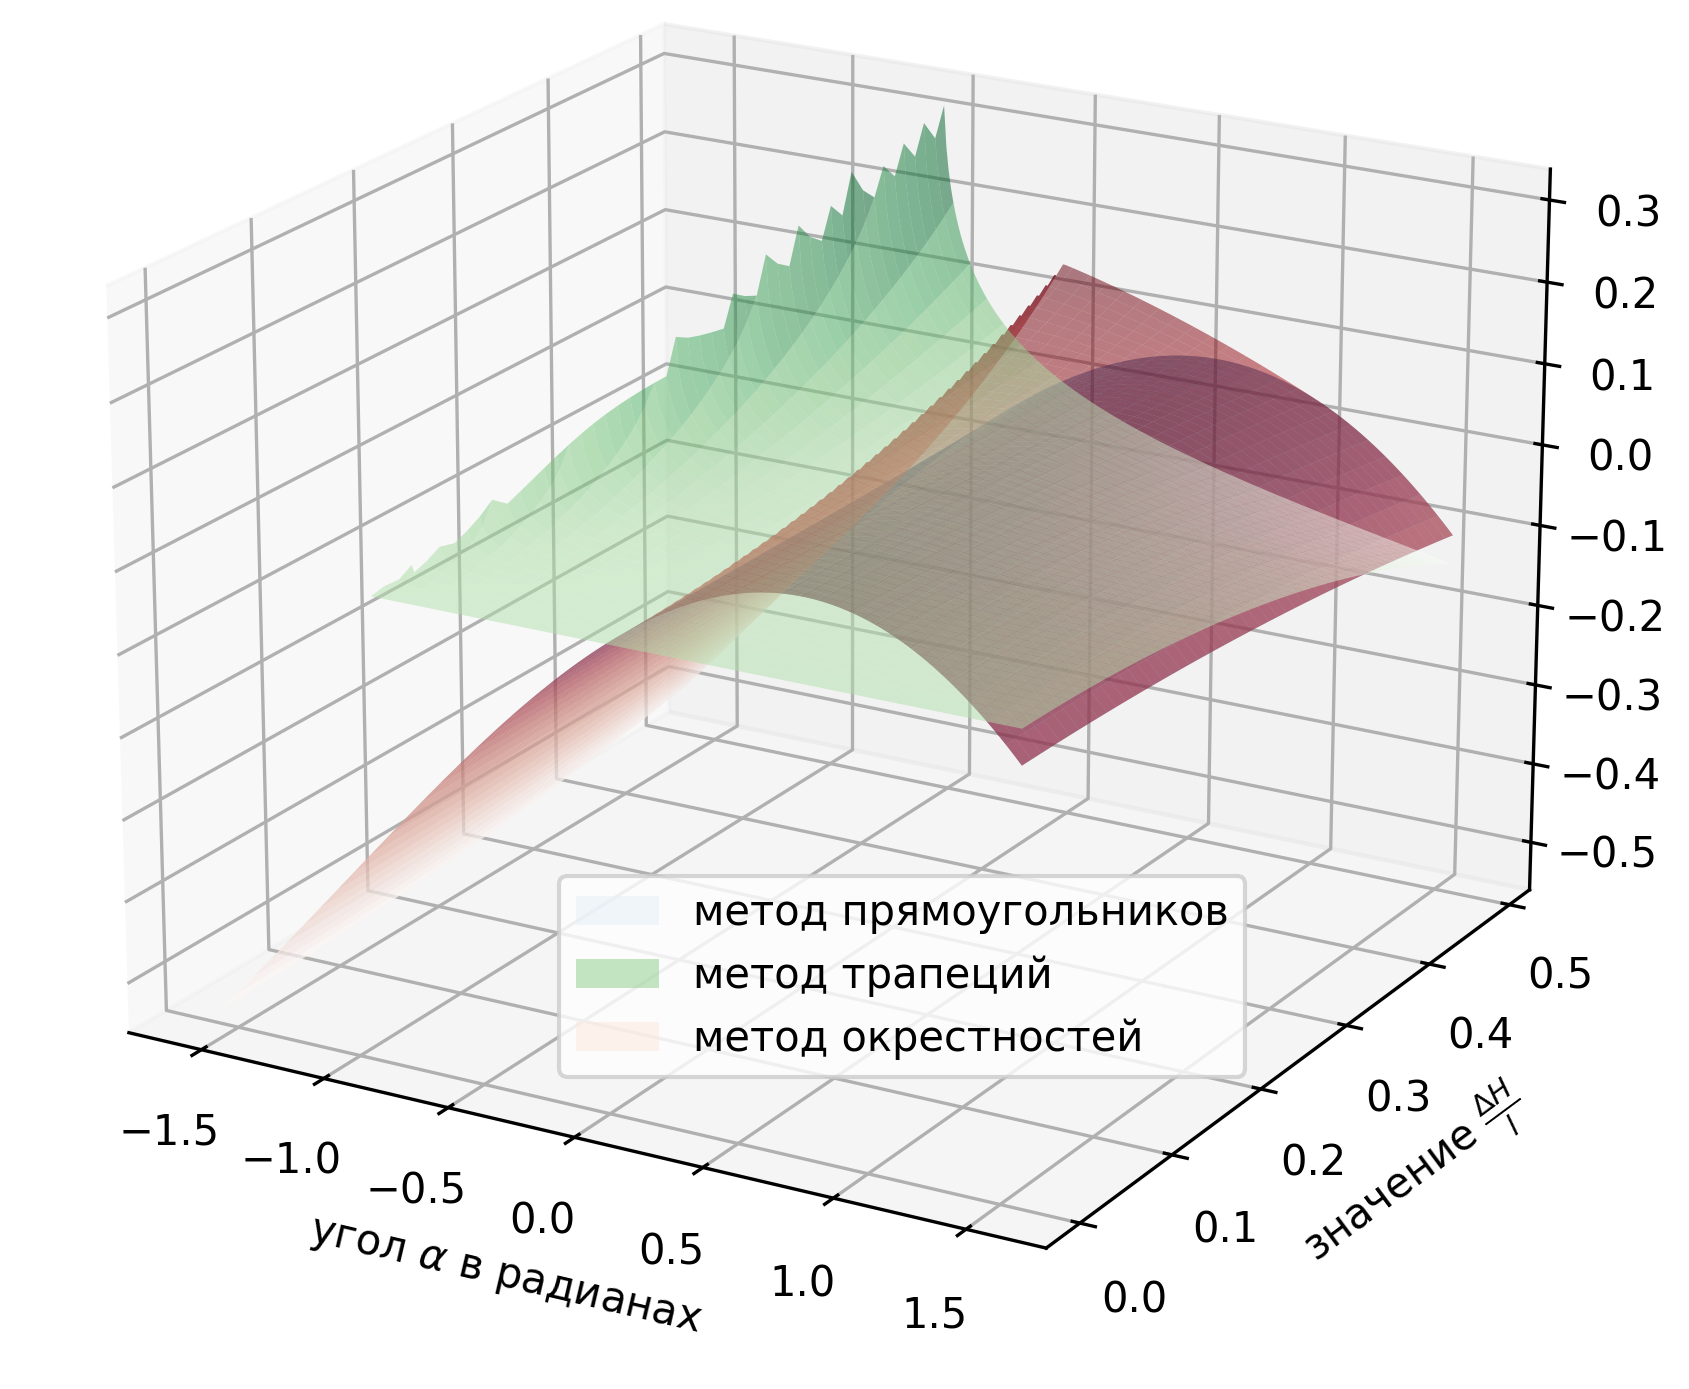
\includegraphics[width=0.8\textwidth]{pics/remesh_3d_chart.png}
\captionstyle{normal}\caption{Графики поверхностей $\delta_i^r(\alpha, \frac{\Delta H}{l})$, $\delta_i^t(\alpha, \frac{\Delta H}{l})$, $\delta_i^o(\alpha, \frac{\Delta H}{l})$ при фиксированном значении $H = \frac{l}{2}$.}
\label{fig:text_1_remesh_3d_main_chart}
\end{figure}

Из рис.~\ref{fig:text_1_remesh_3d_main_chart} можно отметить, что при $\Delta H = 0$ метод трапеций по определению абсолютно точен.
Также отметим, что при $\Delta H = 0$ отклонения $\delta_i^r$ и $\delta_i^o$ практически совпадают.

Построим дополнительно два графика зависимостей $\delta_i^r$, $\delta_i^t$, $\delta_i^o$ от $\frac{\Delta H}{l}$ при фиксированных значениях $\alpha = 0,5$ (для выпуклой сетки) и $\alpha = -0,5$ (для вогнутой сетки) (см. рис.~\ref{fig:text_1_remesh_fix_alfa_chart}).
Из рисунка видно, что метод трапеций перестроения поверхности при небольших значениях $\frac{\Delta H}{l}$ наиболее точен, а точность методов прямоугольников и окрестностей достаточно близки.

\begin{figure}[ht]
\setcaptionmargin{5mm}
\onelinecaptionsfalse % if the caption is multiline
%\onelinecaptionstrue  % if the caption is one-line
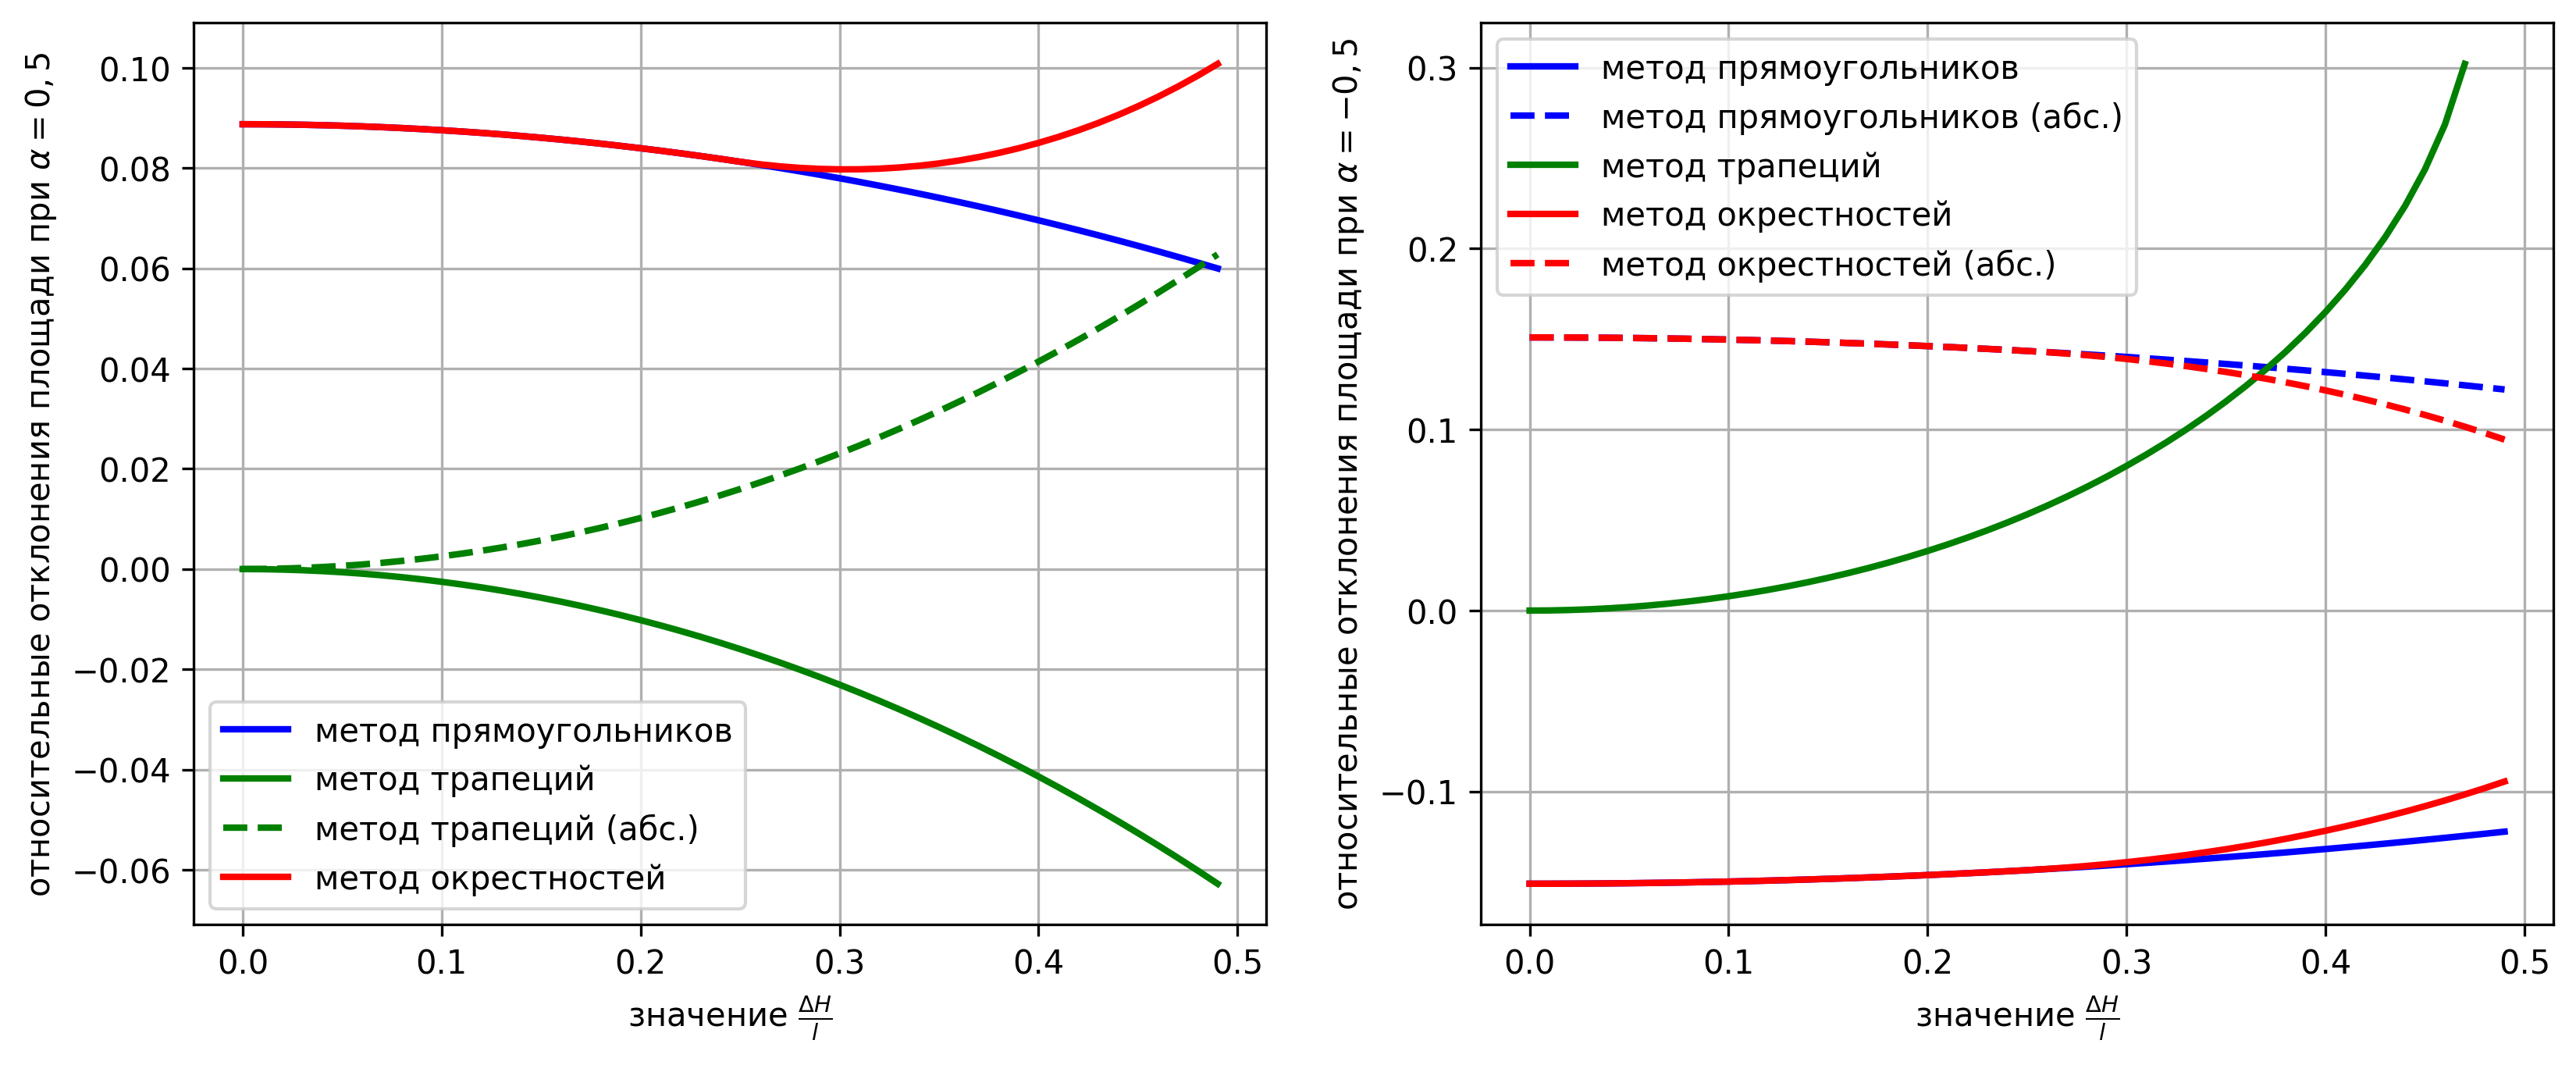
\includegraphics[width=1.0\textwidth]{pics/remesh_fix_alfa_chart.png}
\captionstyle{normal}\caption{Графики поверхностнй $\delta_i^r(\frac{\Delta H}{l})$, $\delta_i^t(\frac{\Delta H}{l})$, $\delta_i^o(\frac{\Delta H}{l})$ при фиксированных значениях $\alpha = 0,5$ (слева) и $\alpha = -0,5$ (справа).}
\label{fig:text_1_remesh_fix_alfa_chart}
\end{figure}

%--------------------------------------------------------------------------------------------------------------------------------

\section{Ozenki sglazhivaniya острых пиков и впадин}

Приведем оценки сглаживания острых пиков и впадин для рассмотренных методов перестроения сетки (методы прямоугольников, трапеций и окрестностей).
Для этого будем рассматривать расчетную сетку с одинаковыми ячейками-отрезками длины $l$.

Для оценки сглаживания острых пиков будем считать, что сетка является абсолютно плоской за исключением двух соседних ячеек, которые образуют острый пик с углом $2 \alpha$ (см. рис.~\ref{fig:text_1_remesh_2d_peak_cavern_general} слева).
Аналогично для оценки сглаживания впадин будем считать, что сетка является абсолютно плоской за исключением двух соседних ячеек, которые образуют впадину с углом $2 \alpha$ (см. рис.~\ref{fig:text_1_remesh_2d_peak_cavern_general} справа)

\begin{figure}[ht]
\setcaptionmargin{5mm}
%\onelinecaptionsfalse % if the caption is multiline
\onelinecaptionstrue  % if the caption is one-line
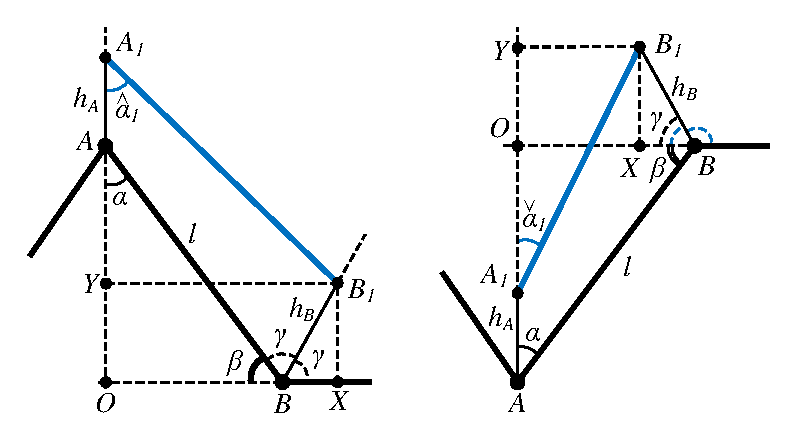
\includegraphics[width=0.8\textwidth]{./pics/peak-cavern-general.pdf}
\captionstyle{normal}\caption{Оценка сглаживания угла при остром пике (слева) и при впадине (справа).}
\label{fig:text_1_remesh_2d_peak_cavern_general}
\end{figure}

Во всех трех методах (прямоугольников, трапеций и окрестностей) направления смещения узлов совпадают (и лежат на биссектрисах углов, образованных соседними ячейками), поэтому будем рассматривать задачу сглаживания угла при остром пике и при впадине для произвольных смещений узлов $A$ и $B$.
Для этого докажем следующие леммы.

\begin{lemma}\label{lem:text_1_peak_smooth}
При перемещении узлов $A$ и $B$ -- узлов одной из сторон острого пика -- вдоль биссектрис углов, образованных инцидентными ячейками, на расстояния $h_A$ и $h_B$ соответственно (см. рис.~\ref{fig:text_1_remesh_2d_peak_cavern_general} слева) значение сглаженного угла $\angle OA_1B_1 = \hat{\alpha}_1$ выражается через $\angle OAB = \alpha$ следующим образом:
\begin{equation}\label{eqn:text_1_envelope_alpha1_peak}
\hat{\alpha}_1(h_A, h_B) = \arctg \frac{l \sin \alpha + h_B \cos \gamma}{l \cos \alpha + h_A - h_B \sin \gamma}	
\end{equation}
\end{lemma}

Выразим через $\alpha$ остальные углы: $\beta = \frac{\pi}{2} - \alpha$, $\gamma = \frac{\pi}{4} + \frac{\alpha}{2}$.
Через углы $\alpha$ и $\gamma$ находим $OA = l \cos \alpha$, $OB = l \sin \alpha$, $BX = h_B \cos \gamma$, $B_1X = h_B \sin \gamma = OY$, откуда получаем $YB_1 = OB + BX = l \sin \alpha + h_B \cos \gamma$, $YA_1 = OA + AA_1 - OY = l \cos \alpha + h_A - h_B \sin \gamma$, откуда получаем $\hat{\alpha}_1(h_A, h_B) = \arctg \frac{YB_1}{YA_1}$, что приводит к \eqref{eqn:text_1_envelope_alpha1_peak}.
$\blacksquare$\\

\begin{lemma}\label{lem:text_1_cavern_smooth}
При перемещении узлов $A$ и $B$ -- узлов одной из сторон впадины -- вдоль биссектрис углов, образованных инцидентными ячейками, на расстояния $h_A \le AO$ и $h_B$ соответственно (см. рис.~\ref{fig:text_1_remesh_2d_peak_cavern_general} справа) значение сглаженного угла $\angle OA_1B_1 = \check{\alpha}_1$ выражается через $\angle OAB = \alpha$ следующим образом:
\begin{equation}\label{eqn:text_1_envelope_alpha1_cavern}
\check{\alpha}_1(h_A, h_B) = \arctg \frac{l \sin \alpha - h_B \cos \gamma}{l \cos \alpha - h_A + h_B \sin \gamma}
\end{equation}
при ограничениях на угол $\alpha$
\begin{equation}\label{eqn:text_1_envelope_alpha1_cavern2}
\arcsin \frac{h_B \left( \sqrt{8 l^2 + h_B^2} - h_B \right)}{4 l^2} \le \alpha \le \arccos \frac{h_A}{l}
\end{equation}
\end{lemma}

Выразим через $\alpha$ остальные углы: $\beta = \frac{\pi}{2} - \alpha$, $\gamma = \frac{\pi}{4} + \frac{\alpha}{2}$.
Через углы $\alpha$ и $\gamma$ находим $OA = l \cos \alpha$, $OB = l \sin \alpha$, $BX = h_B \cos \gamma$, $B_1X = h_B \sin \gamma = OY$, откуда получаем $YB_1 = OB - BX = l \sin \alpha - h_B \cos \gamma$, $YA_1 = OA - AA_1 + OY = l \cos \alpha - h_A + h_B \sin \gamma$, откуда получаем $\check{\alpha}_1(h_A, h_B) = \arctg \frac{YB_1}{YA_1}$, что приводит к \eqref{eqn:text_1_envelope_alpha1_cavern}.

Рассмотрим дополнительные условия применимости формулы \eqref{eqn:text_1_envelope_alpha1_cavern}.

Условие $h_A \le AO$ равносильно $\alpha \le \arccos \frac{h_A}{l}$.

Требованием на отсутствие самопересечения сетки является условие $BX \le OB$, то есть $h_B \cos \gamma \le l \sin \alpha$.
Подставляя явное выражение для $\cos \gamma$, получим
\begin{equation}
	h_B \frac{1}{\sqrt{2}} \left( \cos \frac{\alpha}{2} - \sin \frac{\alpha}{2} \right) \le l \sin \alpha
\end{equation}

Так как $\alpha < \frac{\pi}{2}$, то обе части неравенства положительные, поэтому возведем их в квадрат, и после преобразований получим
\begin{equation}\label{eqn:text_1_envelope_find_alpha3}
	1 - \sin \alpha \le 2 \left( \frac{l}{h_B} \right)^2 \sin^2 \alpha
\end{equation}

Введя обозначение $p = 2 \left( \frac{l}{h_B} \right)^2$ и решая квадратное неравенство \eqref{eqn:text_1_envelope_find_alpha3} относительно $\sin \alpha$, получим условие $\alpha \ge \arcsin \frac{\sqrt{4p + 1} - 1}{2p}$, что в сококупности с условием $\alpha \le \arccos \frac{h_A}{l}$ приводит к \eqref{eqn:text_1_envelope_alpha1_cavern2}.
$\blacksquare$\\

\begin{figure}[ht]
\setcaptionmargin{5mm}
\onelinecaptionsfalse % if the caption is multiline
%\onelinecaptionstrue  % if the caption is one-line
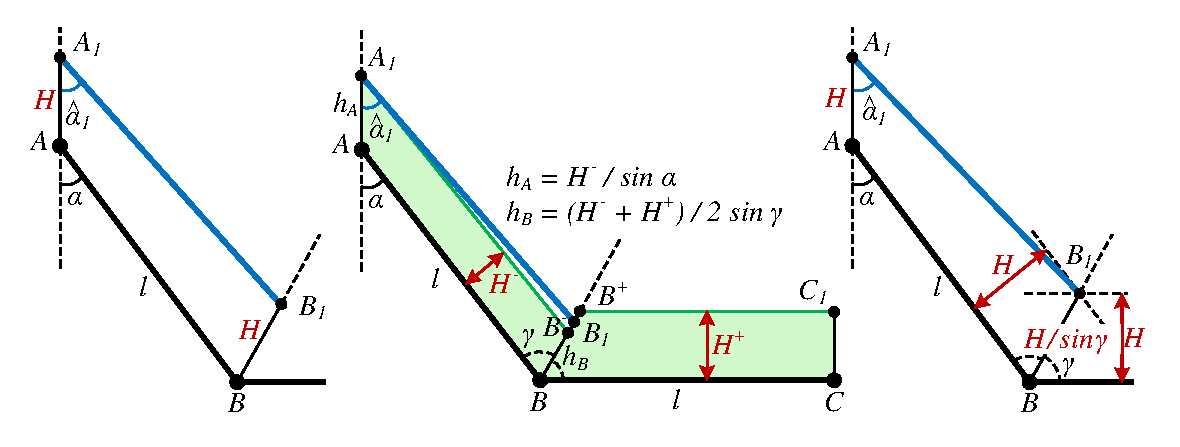
\includegraphics[width=1.0\textwidth]{./pics/peak-methods.pdf}
\captionstyle{normal}\caption{Сглаживание пика при методах прямоугольников (слева), трапеций (в центре), окрестностей (справа).}
\label{fig:text_1_remesh_2d_peak_methods}
\end{figure}

\begin{figure}[ht]
\setcaptionmargin{5mm}
%\onelinecaptionsfalse % if the caption is multiline
\onelinecaptionstrue  % if the caption is one-line
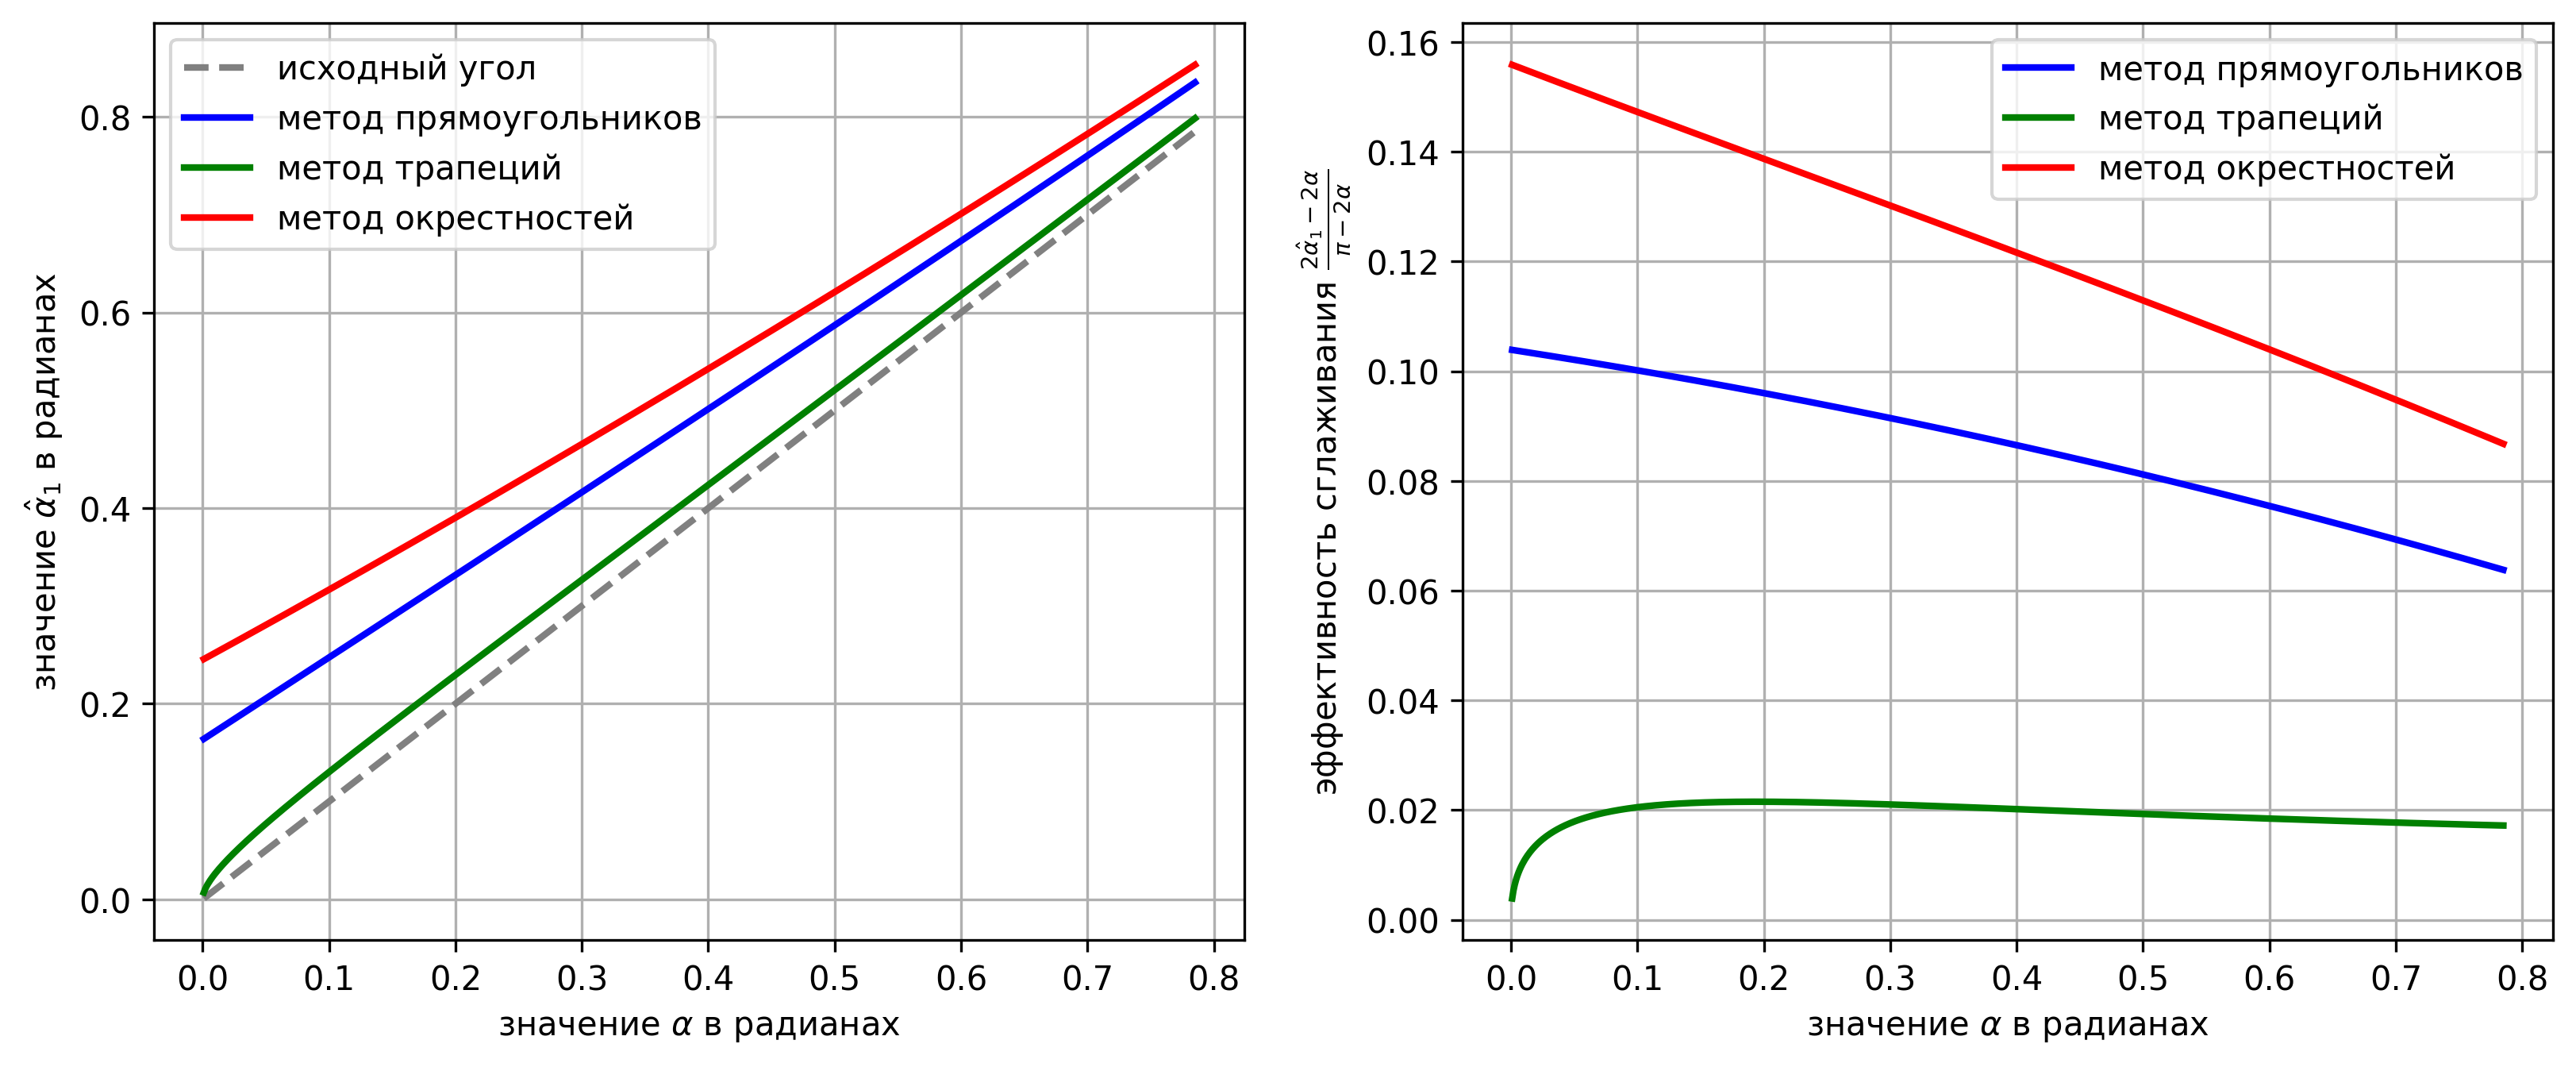
\includegraphics[width=1.0\textwidth]{./pics/peak-methods-chart.png}
\captionstyle{normal}\caption{Сравнение сглаживания острого пика для методов прямоугольников, трапеций и окрестностей.}
\label{fig:text_1_remesh_2d_peak_methods_chart}
\end{figure}

На основе Леммы~\ref{lem:text_1_peak_smooth} получим оценки сглаживания угла при остром пике при условии постоянного значения $H$ во всех ячейках сетки.

Для метода прямоугольников имеем $h_A = h_B = H$ (см. рис~\ref{fig:text_1_remesh_2d_peak_methods} слева).

Для метода трапеций необходимо сначала найти высоты трапеций $AA_1B^{-}B$ и $CC_1B^{+}B$ с рис.~\ref{fig:text_1_remesh_2d_peak_methods} в центре из условия равенства площадей этих трапеций значению $lH$.
Высоты этих трапеций $H^{-}$ и $H^{+}$ получаются с помощью решения квадратного уравнения.
Тогда $h_A = \frac{H^{-}}{\sin \alpha}$, $h_B = \frac{H^{-} + H^{+}}{2 \sin \gamma}$.

В случае метода окрестностей $h_A = H$,  $h_B = \frac{H}{\sin \gamma}$ (см. рис.~\ref{fig:text_1_remesh_2d_peak_methods} справа).

На рис.~\ref{fig:text_1_remesh_2d_peak_methods_chart} приведены графики сравнения методов прямоугольников, трапеций и окрестностей в применении к сглаживанию острых пиков.
При этом используется фиксированная величина смещения ячейки $H = \frac{l}{4}$.
На графике слева показана зависимость изменения сглаженного угла $\hat{\alpha}_1$ от $\alpha$.
На графике справа показана эффективность сглаживания, выраженная формулой $\frac{2 \hat{\alpha}_1 - 2 \alpha}{\pi - 2 \alpha}$ (значение 1 означает полное сглаживание пика до угла $\hat{\alpha}_1 = \frac{\pi}{2}$).

Можно отметить, что наиболее эффективное сглаживание угла $\alpha$ обеспечивает метод окрестностей.
Дополнительно заметим, что использование метода трапеций для малых углов $\alpha$ приводит к неконтролируемому росту $h_A$, что делает применение этого метода неприемлемым.

\begin{figure}[ht]
\setcaptionmargin{5mm}
\onelinecaptionsfalse % if the caption is multiline
%\onelinecaptionstrue  % if the caption is one-line
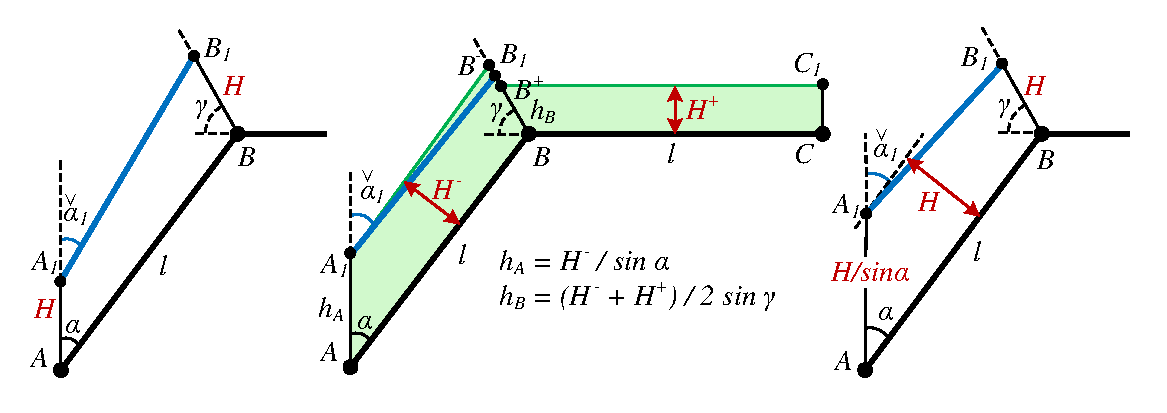
\includegraphics[width=1.0\textwidth]{./pics/cavern-methods.pdf}
\captionstyle{normal}\caption{Сглаживание впадины при методах прямоугольников (слева), трапеций (в центре), окрестностей (справа).}
\label{fig:text_1_remesh_2d_cavern_methods}
\end{figure}

\begin{figure}[ht]
\setcaptionmargin{5mm}
%\onelinecaptionsfalse % if the caption is multiline
\onelinecaptionstrue  % if the caption is one-line
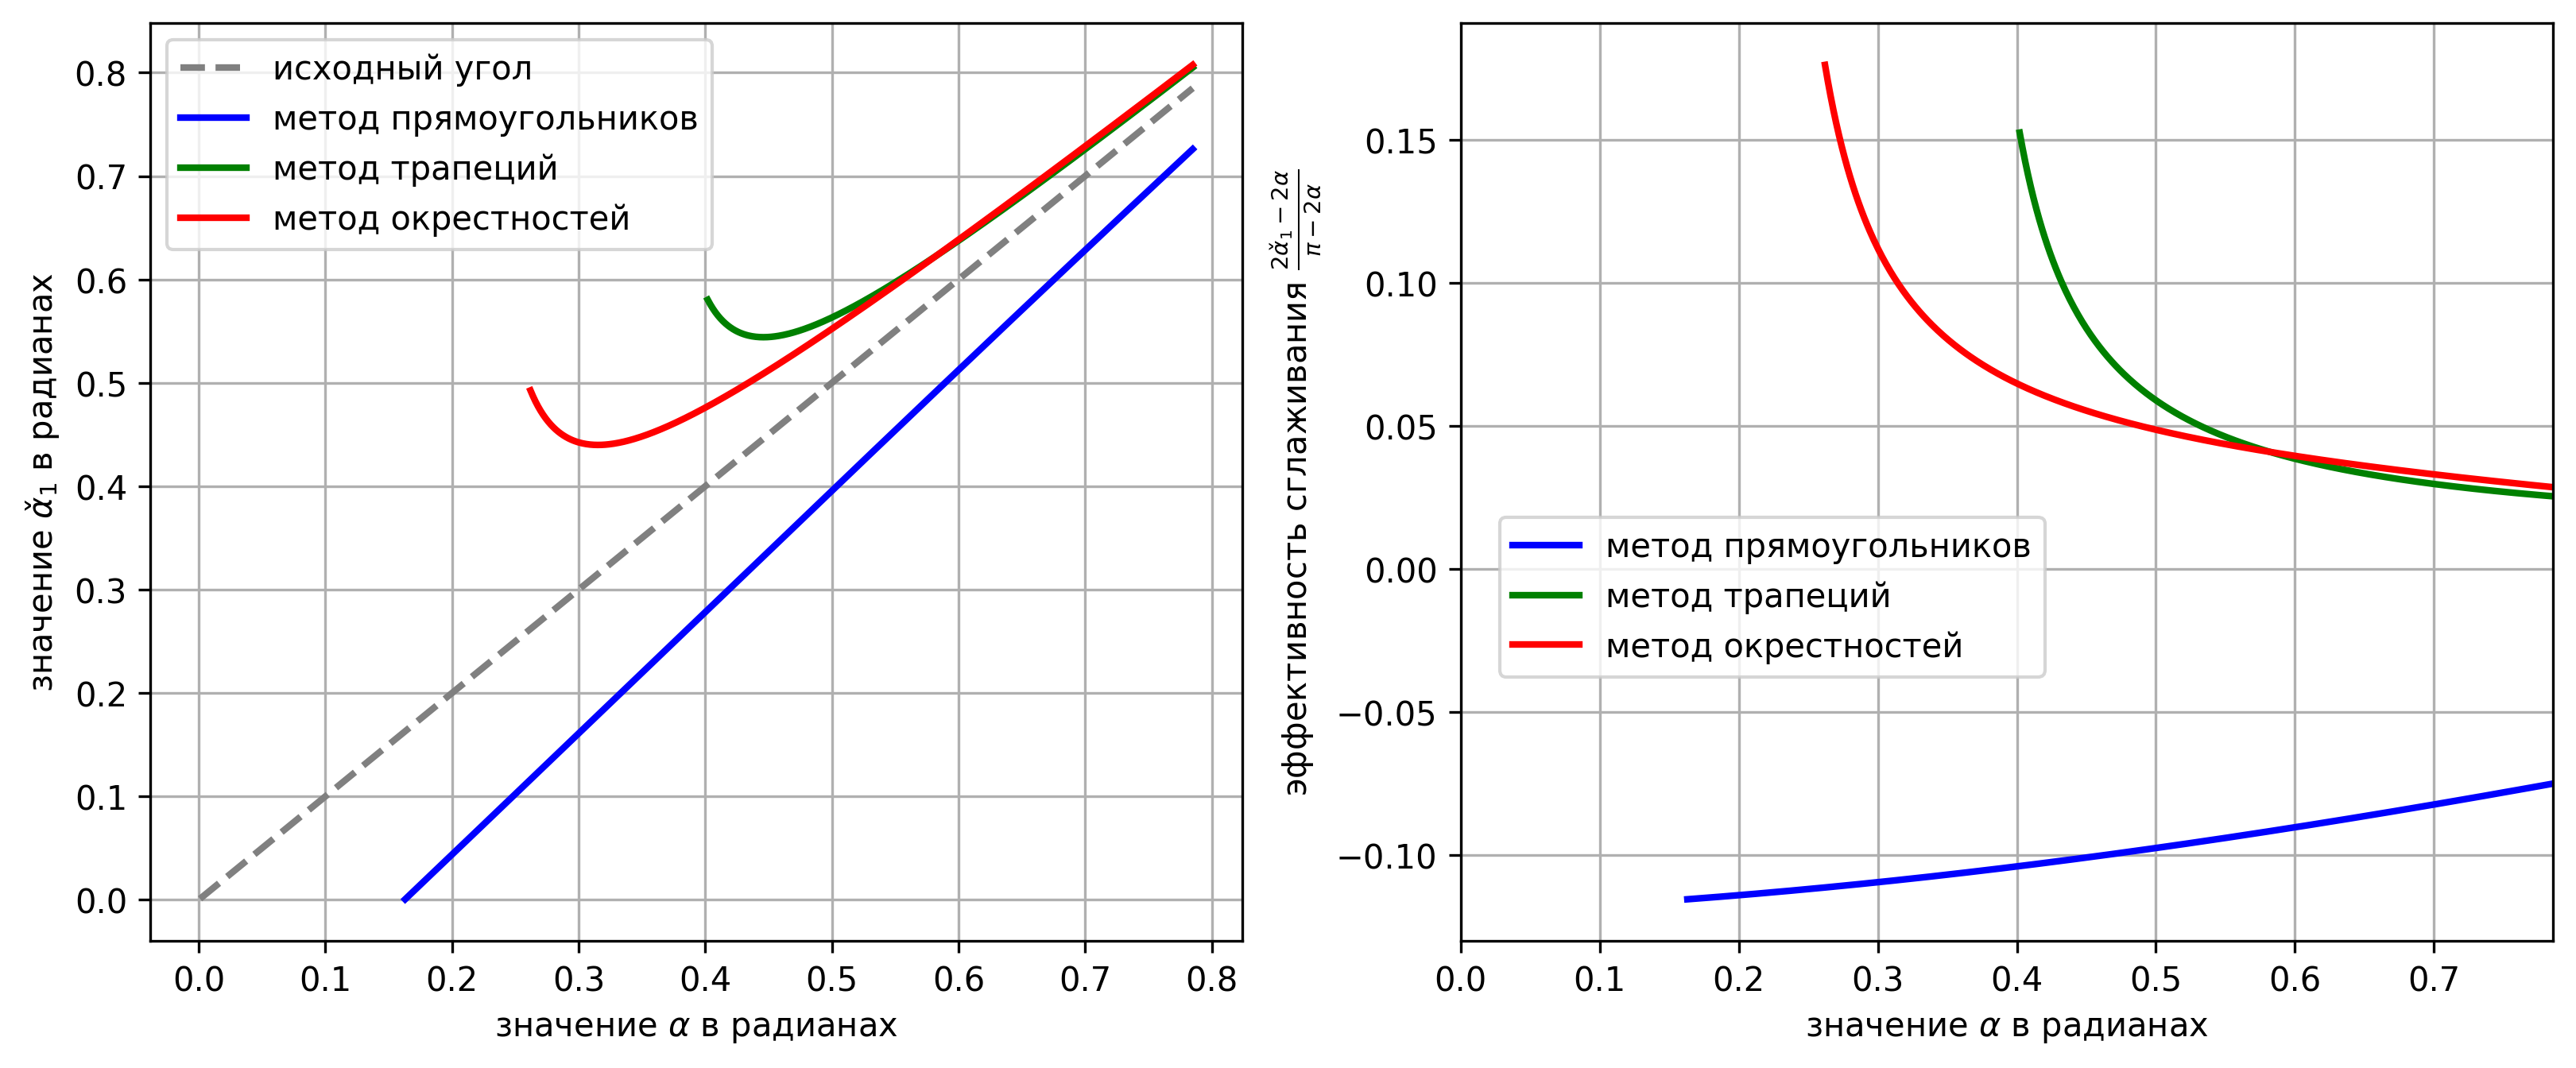
\includegraphics[width=1.0\textwidth]{./pics/cavern-methods-chart.png}
\captionstyle{normal}\caption{Сравнение сглаживания впадины для методов прямоугольников, трапеций и окрестностей.}
\label{fig:text_1_remesh_2d_cavern_methods_chart}
\end{figure}

На основе Леммы~\ref{lem:text_1_cavern_smooth} получим оценки сглаживания угла при впадине при условии постоянного значения $H$ во всех ячейках сетки.

Для метода прямоугольников имеем $h_A = h_B = H$ (см. рис~\ref{fig:text_1_remesh_2d_cavern_methods} слева).

Для метода трапеций необходимо сначала найти высоты трапеций $AA_1B^{-}B$ и $CC_1B^{+}B$ с рис.~\ref{fig:text_1_remesh_2d_cavern_methods} в центре из условия равенства площадей этих трапеций значению $lH$.
Высоты этих трапеций $H^{-}$ и $H^{+}$ получаются с помощью решения квадратного уравнения.
Тогда $h_A = \frac{H^{-}}{\sin \alpha}$, $h_B = \frac{H^{-} + H^{+}}{2 \sin \gamma}$.

В случае метода окрестностей $h_A = \frac{H}{\sin \alpha}$,  $h_B = H$ (см. рис.~\ref{fig:text_1_remesh_2d_cavern_methods} справа).

На рис.~\ref{fig:text_1_remesh_2d_cavern_methods_chart} приведены графики сравнения методов прямоугольников, трапеций и окрестностей в применении к сглаживанию впадин.
При этом используется фиксированная величина смещения ячейки $H = \frac{l}{4}$.
На графике слева показана зависимость изменения сглаженного угла $\check{\alpha}_1$ от $\alpha$.
На графике справа показана эффективность сглаживания, выраженная формулой $\frac{2 \check{\alpha}_1 - 2 \alpha}{\pi - 2 \alpha}$ (значение 1 означает полное сглаживание пика до угла $\hat{\alpha}_1 = \frac{\pi}{2}$).

Можно отметить, что метод прямоугольников не сглаживает угол, а наоборот, делает его еще более острым (значение эффективности сглаживания меньше нуля).
Метод трапеций показывает лучшую эффективность сглаживания, но с меньшей областью применимости.

%--------------------------------------------------------------------------------------------------------------------------------

\section{Conclusion}

Из приведенных оценок точности методов перестроения поверхностной сетки (см. рис.~\ref{fig:text_1_remesh_3d_main_chart}), а также способности сглаживания острых пиков (см. рис.~\ref{fig:text_1_remesh_2d_peak_methods_chart}) и впадин (см. рис.~\ref{fig:text_1_remesh_2d_cavern_methods_chart}) можно сделать следующие выводы.
Метод трапеций перестроения сетки является более точным, точность методов прямоугольников и окрестностей практически совпадают при небольших значениях и изменениях $H$.
С точки зрения сглаживания дефектов сетки метод трапеций неприменим, так как приводит к неконтролируемому росту острых пиков.
Метод прямоугольников неэффективен при сглаживании острых пиков, и не способен сглаживать впадины.
Таким образом, метод окрестностей перестроения является оптимальным с точки зрения точности перестроения и способности сглаживания дефектов сетки.

%--------------------------------------------------------------------------------------------------------------------------------

\begin{acknowledgments}
Работа выполнена в рамках государственного задания НИЦ «Курчатовский институт».
\end{acknowledgments}

%
% The Bibliography
%

\begin{thebibliography}{99}

\bibitem{Raj}
\refitem{article}
L.~Prince~Raj, K.~Yee, and R.~S.~Myong, \textquotedblleft Sensivity of ice and aerodynamic performance degradation to critical physical and modeling parameters affecting airfoil icing\textquotedblright, Aerospace Sci. Technol. \textbf{98}, 105659-1--46 (2020). https://doi.org/10.1016/j.ast.2019.105659

\bibitem{Martini}
\refitem{article}
F.~Martini, H.~Ibrahim, L.~T.~C. Montoya, P.~Rizk, and A.~Ilinca, \textquotedblleft Turbulence modeling of iced wind turbine airfoils\textquotedblright, Energies \textbf{15}, 8325-1--21 (2022). https://doi.org/10.3390/en15228325

\bibitem{Koshelev}
\refitem{article}
K.~B.~Koshelev, V.~G.~Melnikova, and S.~V.~Strijhak, \textquotedblleft Development of ice-foam solver for modeling ice accretion\textquotedblright, Tr. Inst. Sist. Program. RAN \textbf{32}, 217--234 (2020). https://doi.org/10.15514/ISPRAS-2020-32(4)-16

\bibitem{Sorokin}
\refitem{article}
K.~E.~Sorokin, P.~M.~Byvaltsev, A.~A.~Aksenov, S.~V.~Zhluktov, D.~V.~Savitskiy, A.~A.~Babulin, and V.~I.~Shevyakov, \textquotedblleft Numerical simulation of ice accretion if FlowVision sotfware\textquotedblright, Comput. Res. Model. \textbf{12}, 83--96 (2020). https://doi.org/10.20537/2076-7633-2020-12-1-83-96

\bibitem{Galanov}
\refitem{article}
N.~G.~Galanov, A.~V.~Sarazov, R.~N.~Zhukov, and A.~S.~Kozelkov, \textquotedblleft Application of various ice accretion simulation approaches in the LOGOS software package\textquotedblright, J. Phys.: Conf. Ser. \textbf{2099}, 012029-1--8 (2021). https://doi.org/10.1088/1742-6596/2099/1/012029

\bibitem{Bartkus}
\refitem{article}
T.~P.~Bartkus, P.~M.~Struk, and J.-C.~Tsao, “Evaluation of a thermodynamic ice-crystal icing model using experimental ice accretion data,” in \textit{Proceedings of the Atmospheric and Space Environments Conference, 2018, pp. 1--18}. https://doi.org/10.2514/6.2018-4129

\bibitem{Zhang}
\refitem{article}
X.~Zhang, X.~Wu, and J.~Min, “Aircraft icing model considering both rime ice property variability and runback water effect,” Int. J. Heat Mass Transfer \textbf{104}, 510--516 (2017). https://doi.org/10.1016/j.ijheatmasstransfer.2016.08.086

\bibitem{Pena}
\refitem{article}
D.~Pena, Y.~Hoarau, and E.~Laurendeau, “A single step ice accretion model using level-set method,” J. Fluids Struct. \textbf{65}, 278--294 (2016). https://doi.org/10.1016/j.jfluidstructs.2016.06.001

\bibitem{Beaugendre}
\refitem{misc}
H.~Beaugendre, \textquotedblleft A PDE-based approach to in-flight ice accretion\textquotedblright, PhD Thesis (Dep. of Mech. Eng., McGill Univ., Montr\'eal, Qu\'ebec, 2003).

\bibitem{Tong}
\refitem{article}
X.~Tong, D.~Thompson, Q.~Arnoldus, E.~Collins, and E.~Luke, \textquotedblleft Three-dimensional  surface evolution and mesh deformation for aircraft icing applications\textquotedblright, J. of Aircraft {\bf 54}, 1047--1063 (2017). https://doi.org/10.2514/1.C033949

\bibitem{Rybakov}
\refitem{article}
A.~A.~Rybakov and S.~S.~Shumilin, \textquotedblleft Approximate  methods of the surface mesh deformation in two-dimensional case\textquotedblright, Lobachevskii J. Math. {\bf 40}, 1848--1852 (2019). https://doi.org/10.1134/S1995080219110258

\bibitem{Meshcheryakov}
\refitem{article}
A.~O.~Meshcheryakov, and A.~A.~Rybakov, \textquotedblleft Evolution of the surface computational mesh in the ice accretion process\textquotedblright, Lobachevskii J. Math. {\bf 44}, 361--378 (2023). https://doi.org/10.1134/S1995080223110367

\end{thebibliography}
\end{document}
